%% Springer Nature article (sn-jnl class, numbered references).
%% Compile with pdfLaTeX + BibTeX inside the Springer Nature Overleaf template (upload paper.tex, references.bib and figures/).
\documentclass[pdflatex,sn-mathphys-num]{sn-jnl}

\usepackage{graphicx}
\usepackage{amsmath,amssymb,amsfonts}
\usepackage{amsthm}
\usepackage{booktabs}
\usepackage{array}
\usepackage{tabularx}
\usepackage{multirow}
\usepackage{xcolor}
\usepackage{algorithm}
\usepackage{algorithmicx}
\usepackage{algpseudocode}
\usepackage[section]{placeins}
\newcolumntype{Y}{>{\raggedright\arraybackslash}X}
\newcolumntype{C}{>{\centering\arraybackslash}X}
\raggedbottom

\theoremstyle{thmstyleone}
\newtheorem{proposition}{Proposition}
\newtheorem{lemma}{Lemma}
\theoremstyle{thmstylethree}
\newtheorem{remark}{Remark}

\begin{document}

\title[Benign-Reference Memory Audit for Federated Continual Intrusion Detection]{Removing Persistent Label Poisoning from Replay Memory in Federated Class-Incremental Intrusion Detection with a Conformal Benign-Reference Audit}

\author*[1]{\fnm{Saneedullah}}\email{i232568@isb.nu.edu.pk}
\author[1]{\fnm{Ahmed} \sur{Bilal}}\email{i232581@isb.nu.edu.pk}

\affil*[1]{\orgdiv{Department of Data Science}, \orgname{FAST National University of Computer and Emerging Sciences}, \orgaddress{\city{Islamabad}, \country{Pakistan}}}

\abstract{In federated class-incremental intrusion detection, client replay memories prevent forgetting but also retain poisoned records: when clients relabel a newly arriving attack family as benign, the flipped records remain in replay and mislead the global model after the attackers withdraw. We formalise this persistent label-poisoning threat and propose the Benign-Reference Memory Audit (BRMA). At the end of each stage, the server fits a tied-covariance Gaussian model to first-stage benign traffic and to client attack-labelled traffic, scores every benign-labelled replay record by a likelihood ratio, and removes records above a split-conformal threshold that provably bounds the removal rate of genuine benign records by $\alpha$. On CIC-IDS2017 (600 runs), BRMA detects 99.9\% of poisoned memory records with false removals of 4.5--4.7\% at $\alpha=0.05$ and reduces the attack effect of three to five colluding clients from 0.525--0.586 to 0.0006--0.0022, outperforming random deletion, EWC, small-loss filtering and median aggregation. Adaptive attackers who flip only the records that look most benign to their own copy of the audit are still detected at 99.98\% (672 runs). On TON\_IoT, the protected learner achieves 89.1\% macro-F1 and 97.1\% accuracy, exceeding the 74.49\% F1 reported by a recent federated class-incremental system. Where DDoS and normal flows overlap, a combined audit (BRMA-C) that adds a conformal test on the model's attack score raises detection from 59\% to above 99\% and removes 91--97\% of the attack effect left by BRMA on unseen seeds, while a model-only audit fails on CIC-IDS2017 because the model itself is poisoned.}

\keywords{federated learning, continual learning, intrusion detection, label poisoning, replay memory, conformal prediction}

\maketitle

%=====================================================================
\section{Introduction}\label{sec:intro}
Network intrusion detection systems (NIDS) face two pressures at once. New attack families appear continuously, so a deployed detector must learn them without forgetting the families it already knows, which is the problem studied by class-incremental continual learning \cite{delange,icarl}. At the same time, the traffic needed to learn them is spread over organisations that cannot share it, which is why federated learning (FL) has become a common way to train detectors jointly \cite{fedavg,kairouz,agrawal}. Recent federated class-incremental intrusion detection systems combine the two and keep a small replay memory on every client \cite{carillo,wu}. Replay is the most reliable protection against forgetting in this setting \cite{der,cerasuolo}, and Carillo et al.\ report 74.49\% F1 over all classes on TON\_IoT with rehearsal and bias correction \cite{carillo}.

These systems assume that every client labels its traffic honestly. Carillo et al.\ list robustness against adversarial threats as future work \cite{carillo}, and Wu et al.\ state that malicious clients are outside their scope \cite{wu}. Poisoning studies of federated IDS, in turn, keep the set of classes fixed. Lavaur et al.\ find that a single label-flipping client has little effect and that the global model recovers quickly once the attack stops \cite{lavaur}, and robust aggregation and client-scoring defences are evaluated on static label spaces \cite{yin,krum,fltrust,wei,lfighter}. A replay memory breaks the recovery argument. Records that were flipped while a new family was being learned are sampled into memory and rehearsed in every later stage, so the poison keeps acting after its source has gone. A centralised preprint shows that flipping labels inside a continual IDS replay buffer can collapse the detector \cite{replaypoison}, but no defence has been proposed for the federated case.

We study this gap and propose the Benign-Reference Memory Audit (BRMA). The idea rests on an asymmetry. A record whose label was flipped from an attack family to benign keeps the features of the attack family. If the server holds statistics of genuine benign traffic from the first stage, before any attack, and statistics of the attack families from records the clients themselves label as attacks, a flipped record looks much more like an attack than like benign traffic, although it carries a benign label. BRMA turns this into a likelihood-ratio score under a tied-covariance Gaussian model \cite{lee2018,ren2019}, sets the removal threshold by split-conformal calibration so that genuine benign records are removed with probability at most $\alpha$ \cite{vovk,bates,angelopoulos}, and lets the reservoir refill the freed slots.

We address three research questions. RQ1: does label poisoning persist in the replay memory of a federated class-incremental detector, and how much of the later damage does the memory explain? RQ2: can a benign-reference conformal audit remove the poisoned records while keeping legitimate learning of new families and the false-alarm rate unchanged? RQ3: how does the audit compare with published defences, and when does it fail?

The paper makes four contributions.
\begin{itemize}
\item A formal model of persistent label poisoning in federated class-incremental intrusion detection, with $k$ coordinated clients that flip a fraction $\rho$ of a newly arriving family to benign and then withdraw, and an attack-effect measure that isolates the damage remaining after withdrawal (Section~\ref{sec:model}).
\item BRMA, a server-side audit with a closed-form score, a finite-sample bound on false removals, a detection-power expression under the Gaussian model, and a cost of one small statistics exchange per stage, together with two extensions: a model-score test (BRMA-M) and a combined audit (BRMA-C) that keeps the same false-removal bound (Section~\ref{sec:method}).
\item An evaluation on CIC-IDS2017 with 600 runs over 12 seeds and five attack strengths, against fine-tuning, EWC, small-loss admission filters, coordinate-wise median aggregation and three memory controls, with six confirmatory tests specified in advance and corrected for multiplicity, followed by a second study of 672 runs with adaptive attackers who know the audit and a fixed-budget loss filter (Sections~\ref{sec:setup} and~\ref{sec:results}).
\item A second evaluation on TON\_IoT, the dataset used by Carillo et al.\ \cite{carillo}, where our learner exceeds the reported F1 by 14.6 points, an analysis of why the Gaussian audit detects only part of the poison when attack and benign flows overlap, and a two-phase study on unseen seeds (843 further runs) showing that BRMA-C closes this gap on TON\_IoT while keeping the CIC-IDS2017 result, whereas a model-only audit fails when the model is poisoned.
\end{itemize}

Section~\ref{sec:related} reviews related work and Section~\ref{sec:model} defines the system and threat model. Section~\ref{sec:method} presents BRMA, Section~\ref{sec:setup} the experimental setup and Section~\ref{sec:results} the results. Section~\ref{sec:discussion} discusses limitations and Section~\ref{sec:conclusion} concludes.

%=====================================================================
\section{Related Work}\label{sec:related}
Continual intrusion detection is studied mostly in the centralised setting. Cerasuolo et al.\ benchmark class-incremental methods on IoT traffic and report 95.30\% F1 on TON\_IoT with optimised packet fields and memory \cite{cerasuolo}, and extend the approach with explainability and cross-network adaptation \cite{cerasuolo2}. Guo et al.\ combine a clustering-based memory with multi-level distillation and report 83.4\% accuracy on CIC-IDS2017 \cite{guo}. Delgado et al.\ compare eight continual strategies in a binary domain-incremental setting and find that replay keeps macro-F1 at 0.92--0.98 \cite{delgado}. Other work adds EWC to graph networks \cite{elgnn}, aligns task heads \cite{ctwa}, discovers unknown DoS attacks before expanding the classifier \cite{ge}, or detects novelty without labels \cite{cnd}. The underlying continual-learning methods are regularisation such as EWC and LwF \cite{ewc,lwf} and rehearsal such as iCaRL and DER++ \cite{icarl,der}; surveys are given in \cite{delange}. All these studies assume clean labels.

Federated class-incremental detectors add the federation. Carillo et al.\ pair FedAvg, FedProx and FedDyn with rehearsal and bias correction on three IoT datasets \cite{carillo}, Wu et al.\ keep client-local replay and distillation and compress the updates \cite{wu}, and Abhijit et al.\ detect rare and newly emerging classes with federated transfer learning \cite{rare}. All three train with honest clients.

Poisoning of federated learning has been studied without class increments. Label flipping by a subset of clients degrades the targeted class \cite{tolpegin}, but in federated IDS the effect of a single attacker is diluted and fades after the attack \cite{lavaur}. Defences either aggregate robustly, for example with Krum or the coordinate-wise median \cite{krum,yin}, score client updates against trusted server data \cite{fltrust,wei}, cluster or filter updates \cite{amm,flzt,lfighter}, or gate updates in an ensemble \cite{prasad}. These defences act on model updates during the attack. They cannot remove poisoned records that already sit in a client's replay memory, and they are evaluated on fixed label spaces. Data-level defences sanitise labels with nearest neighbours \cite{paudice} or keep low-loss samples, which is the usual remedy for noisy labels \cite{itlm,coteach,mentornet,song}. Low-loss filtering also discards hard but legitimate samples, and a newly arriving family is hard to fit by definition.

BRMA borrows from out-of-distribution detection, where class-conditional Gaussian scores with a shared covariance \cite{lee2018} and likelihood ratios \cite{ren2019} detect inputs that do not match their class, and from conformal inference, which gives distribution-free error control for outlier tests \cite{vovk,lei,bates,angelopoulos}. To our knowledge it is the first defence that audits federated replay memories. Table~\ref{tab:related} summarises the positioning.

\begin{table}[htbp]
\caption{Positioning of related studies. Fed.: federated training; CIL: new classes arrive over time; Poison: poisoning evaluated; Memory defence: poisoned records are removed from a replay memory.}\label{tab:related}
\footnotesize
\begin{tabularx}{\textwidth}{@{}p{3.3cm}Ycccc@{}}
\toprule
Study & Focus & Fed. & CIL & Poison & Memory defence\\
\midrule
Carillo et al.\ 2026 \cite{carillo} & Federated incremental NIDS for IoT & yes & yes & no & no\\
Wu et al.\ 2026 \cite{wu} & Communication-efficient federated CIL & yes & yes & no & no\\
Abhijit et al.\ 2025 \cite{rare} & Rare and new classes in FL & yes & yes & no & no\\
Cerasuolo et al.\ 2025 \cite{cerasuolo} & Class-incremental IoT NIDS & no & yes & no & no\\
Guo et al.\ 2025 \cite{guo} & Memory selection and distillation & no & yes & no & no\\
Delgado et al.\ 2026 \cite{delgado} & Domain-incremental IoT NIDS & no & yes & no & no\\
Lavaur et al.\ 2025 \cite{lavaur} & Label flipping in federated IDS & yes & no & yes & no\\
Sameera et al.\ 2025 \cite{wei} & Weibull-based client scoring & yes & no & yes & no\\
Jebreel et al.\ 2024 \cite{lfighter} & Label-flipping defence in FL & yes & no & yes & no\\
Prasad et al.\ 2026 \cite{prasad} & Gated federated ensemble & yes & no & yes & no\\
Ariffin et al.\ 2026 \cite{replaypoison} & Replay-buffer poisoning (preprint) & no & yes & yes & no\\
This work & Conformal audit of replay memory & yes & yes & yes & yes\\
\botrule
\end{tabularx}
\end{table}

%=====================================================================
\section{System Model and Problem Formulation}\label{sec:model}
\subsection{Federated class-incremental learning}
A server and $K$ clients learn over $T$ stages. At stage $t$ client $k$ holds a private set $D_k^t=\{(x_i,\tilde y_i)\}$ of flow records $x_i\in\mathbb{R}^d$ with supplied labels $\tilde y_i$. The set of classes seen so far, $\mathcal{C}_t\supseteq\mathcal{C}_{t-1}$, grows when a new attack family appears, and class $0$ denotes benign traffic, which is present in every stage. The model $f_\theta:\mathbb{R}^d\to\mathbb{R}^{|\mathcal{C}_t|}$ is a multilayer perceptron whose output layer is extended by one row per new class. Each client keeps a replay memory $M_k$ of capacity $B$ filled by reservoir sampling \cite{vitter} during the first pass over each stage; a stored entry $(x^m,\tilde y^m,z^m)$ contains the record, its supplied label and the logits $z^m$ of the model at insertion time. Local training minimises the DER++ objective \cite{der}
\begin{equation}
\mathcal{L}_k(\theta)=\frac{1}{|b|}\sum_{(x,\tilde y)\in b}\ell\big(f_\theta(x),\tilde y\big)+\frac{\lambda_y}{|m|}\sum_{j\in m}\ell\big(f_\theta(x^j),\tilde y^j\big)+\frac{\lambda_z}{|m|}\sum_{j\in m}\frac{\|f_\theta(x^j)_{1:w_j}-z^j\|_2^2}{w_j},
\label{eq:der}
\end{equation}
where $b$ is a batch of current records, $m$ a batch drawn from $M_k$, $\ell$ the cross-entropy and $w_j$ the number of classes known when entry $j$ was stored. After $E$ local epochs the server aggregates by federated averaging \cite{fedavg},
\begin{equation}
\theta^{r+1}=\sum_{k=1}^{K}\frac{n_k}{n}\,\theta_k^{r+1},\qquad n=\sum_k n_k,
\label{eq:fedavg}
\end{equation}
for $R$ rounds per stage, where $n_k$ is the number of records client $k$ trains on.

\subsection{Threat model}
A set $\mathcal{A}$ of $|\mathcal{A}|=k$ clients is malicious. During the attack stage $t_a$, when a target family $c^\ast$ is learned for the first time, each attacker $a\in\mathcal{A}$ relabels a fraction $\rho$ of its own records of $c^\ast$ as benign:
\begin{equation}
\tilde y_i=0\quad\text{for } i\in P_a,\qquad P_a\subseteq\{i\in D_a^{t_a}: y_i=c^\ast\},\qquad |P_a|=\lfloor\rho\, n_{a,c^\ast}\rfloor .
\label{eq:attack}
\end{equation}
The goal is persistent evasion: traffic of $c^\ast$ should still be classified as benign after the attackers have returned to honest behaviour in stages $t>t_a$. The attackers follow the training protocol, know the learning algorithm and the audit, and can coordinate the choice of $P_a$, but they do not alter features, cannot change other clients' data and do not see the audit's random splits. The server aggregates honestly. Following the trusted-bootstrap assumption of FLTrust \cite{fltrust}, the benign records of the first stage are assumed clean, because no attack family has been introduced yet.

We measure the damage that remains after withdrawal. Let $\mathrm{ASR}_t=\Pr(\hat y=0\mid y=c^\ast)$ be the fraction of held-out $c^\ast$ records classified as benign after stage $t$, and $\mathrm{ASR}_t^{\mathrm{clean}}$ the same quantity for the same method and seed without attack. The attack effect is
\begin{equation}
H=\frac{1}{2}\sum_{t\in\{t_a+1,\,t_a+2\}}\big(\mathrm{ASR}_t-\mathrm{ASR}_t^{\mathrm{clean}}\big).
\label{eq:H}
\end{equation}

\subsection{Problem statement}
A memory audit is a rule that, at the end of stage $t$, selects a removal set $\mathcal{D}_k^t\subseteq M_k$ on every client. We seek a rule that minimises $\mathbb{E}[H]$ subject to a bound on the removal of genuine benign records,
\begin{equation}
\Pr\big(x\in\mathcal{D}_k^t \,\big|\, x\in M_k,\ \tilde y=y=0\big)\leq\alpha ,
\label{eq:problem}
\end{equation}
while keeping the macro-F1, the learning of new families and the benign false-alarm rate of the undefended learner. Only benign-labelled records are candidates, because the attack of Eq.~\eqref{eq:attack} only creates false benign labels. Table~\ref{tab:notation} lists the notation.

\begin{table}[htbp]
\caption{Main notation.}\label{tab:notation}
\footnotesize
\begin{tabularx}{\textwidth}{@{}lY@{}}
\toprule
Symbol & Meaning\\
\midrule
$K$, $T$, $R$, $E$ & clients, stages, rounds per stage, local epochs\\
$D_k^t$, $M_k$, $B$ & stage data and replay memory of client $k$, memory capacity\\
$\mathcal{C}_t$, $c^\ast$ & classes seen up to stage $t$, target family of the attack\\
$\mathcal{A}$, $k$, $\rho$ & attacking clients, their number, fraction of $c^\ast$ records flipped\\
$\mathcal{R}$, $\mathcal{Q}$ & benign reference and calibration halves of the stage-1 benign records\\
$\hat\mu_c$, $\hat\Sigma$, $P$ & class means, shrunk shared covariance, precision matrix $\hat\Sigma^{-1}$\\
$s(x)$, $\tau_\alpha$ & BRMA likelihood-ratio score, conformal threshold at level $\alpha$\\
$H$ & attack effect after withdrawal, Eq.~\eqref{eq:H}\\
\botrule
\end{tabularx}
\end{table}

%=====================================================================
\section{Benign-Reference Memory Audit}\label{sec:method}
Figure~\ref{fig:arch} shows the architecture. Clients train with replay and send model updates as usual. Once per stage they also send per-class sufficient statistics, the server fits the BRMA model and calibrates a threshold, and every client audits its own memory with the broadcast statistics. Records never leave the clients.

\begin{figure}[htbp]
\centering
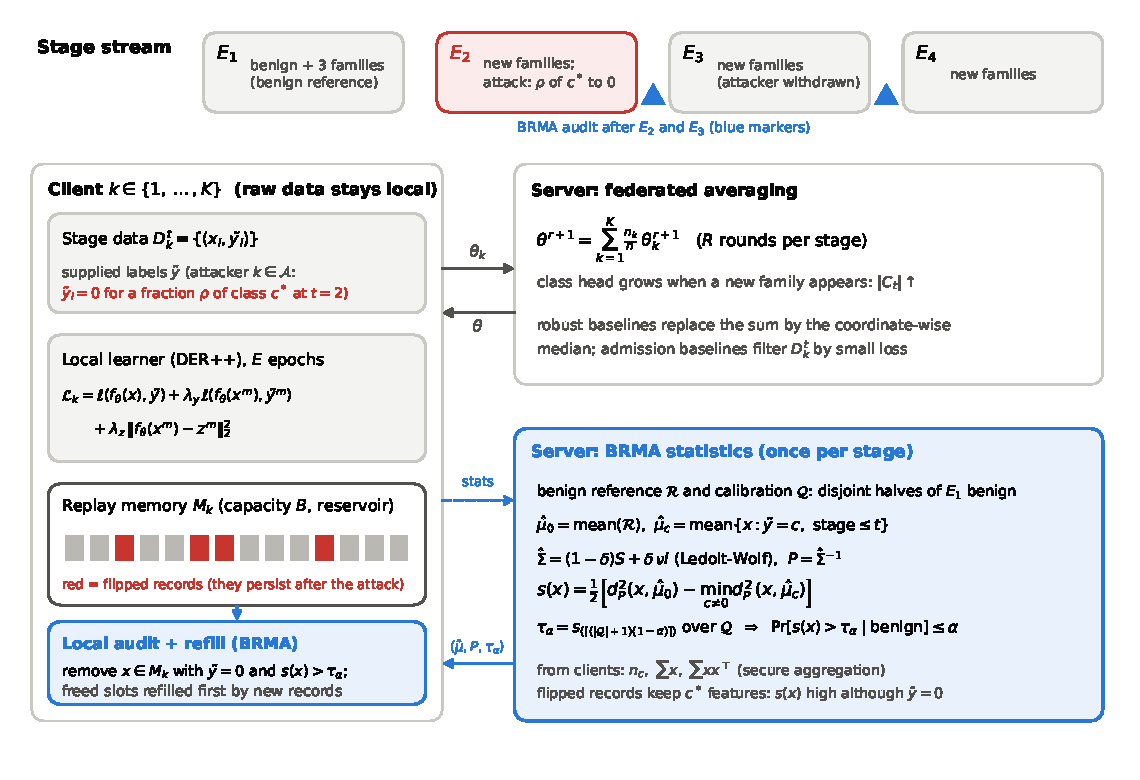
\includegraphics[width=\textwidth]{figures/fig1_architecture.pdf}
\caption{BRMA architecture. Top: the four-stage stream with the attack in stage $E_2$ and audits after $E_2$ and $E_3$. Left: a client with its stage data, DER++ learner, replay memory in which flipped records persist, and the local audit. Right: federated averaging and the server-side BRMA statistics, score and conformal threshold.}\label{fig:arch}
\end{figure}

\subsection{Likelihood-ratio score}
Features are standardised with the mean and standard deviation of the stage-1 records. The stage-1 benign records are split at random into a reference half $\mathcal{R}$ and a calibration half $\mathcal{Q}$. For every attack class $c\in\mathcal{C}_t\setminus\{0\}$ with at least 20 records, the server forms the mean $\hat\mu_c$ of all records that clients labelled $c$ in stages $1,\dots,t$, and $\hat\mu_0$ is the mean of $\mathcal{R}$. A shared covariance is estimated from the pooled within-class deviations with Ledoit--Wolf shrinkage \cite{ledoit},
\begin{equation}
\hat\Sigma=(1-\hat\delta)\,S+\hat\delta\,\hat\nu\, I,\qquad P=\hat\Sigma^{-1},
\label{eq:lw}
\end{equation}
where $S$ is the pooled scatter matrix, $\hat\nu=\mathrm{tr}(S)/d$ and $\hat\delta\in[0,1]$ is the shrinkage intensity that minimises the expected Frobenius loss. Under the model $x\mid c\sim\mathcal{N}(\hat\mu_c,\hat\Sigma)$, the log-likelihood ratio between the most likely attack class and benign is
\begin{equation}
s(x)=\max_{c\neq 0}\log\frac{p(x\mid c)}{p(x\mid 0)}=\frac{1}{2}\Big[d_P^2(x,\hat\mu_0)-\min_{c\neq 0}d_P^2(x,\hat\mu_c)\Big],\qquad d_P^2(x,\mu)=(x-\mu)^{\top}P(x-\mu).
\label{eq:score}
\end{equation}
A large score means that a record labelled benign is much better explained by some attack class.

\begin{lemma}[No contamination]\label{lem:clean}
Under the threat model, the attack of Eq.~\eqref{eq:attack} changes neither $\hat\mu_0$ nor any $\hat\mu_c$ with $c\neq 0$ through flipped records.
\end{lemma}
\begin{proof}
$\hat\mu_0$ is computed from stage-1 benign records, which precede the attack stage. A flipped record carries the label $0$ and therefore never enters the set of records labelled $c$ for any $c\neq 0$; the records of $c^\ast$ that remain are genuine.
\end{proof}

The attack therefore removes records from the $c^\ast$ statistics but cannot shift them towards benign. This is what separates BRMA from defences that learn from the poisoned labels themselves.

\subsection{Conformal threshold and detection power}
Let $s_{(1)}\le\dots\le s_{(n)}$ be the sorted scores of the $n=|\mathcal{Q}|$ calibration records. BRMA uses the split-conformal threshold \cite{vovk,lei}
\begin{equation}
\tau_\alpha=s_{(\lceil (n+1)(1-\alpha)\rceil)}
\label{eq:tau}
\end{equation}
and removes a benign-labelled memory record $x$ when $s(x)>\tau_\alpha$.

\begin{proposition}[False-removal control]\label{prop:fdr}
If the score of a genuine benign memory record is exchangeable with the calibration scores, then $\Pr\big(s(x)>\tau_\alpha\big)\le\alpha$.
\end{proposition}
\begin{proof}
By exchangeability, the rank of $s(x)$ among the $n+1$ scores $\{s(x),s_{(1)},\dots,s_{(n)}\}$ is uniform on $\{1,\dots,n+1\}$ when ties are broken at random. The event $s(x)>s_{(j)}$ with $j=\lceil (n+1)(1-\alpha)\rceil$ requires a rank above $j$, which has probability at most $(n+1-j)/(n+1)\le\alpha$ \cite{bates}.
\end{proof}

The guarantee depends only on the benign side and holds for any model of the attack classes, so a poor attack model costs detection power but not false removals. Exchangeability is an assumption: benign traffic may drift between stages, and Section~\ref{sec:results} checks the realised false-removal rate.

\begin{proposition}[Detection power under the Gaussian model]\label{prop:power}
Let benign and target records follow $\mathcal{N}(\mu_0,\Sigma)$ and $\mathcal{N}(\mu_{c^\ast},\Sigma)$ with known parameters, and let $\Delta^2=(\mu_{c^\ast}-\mu_0)^{\top}\Sigma^{-1}(\mu_{c^\ast}-\mu_0)$. The likelihood-ratio test at level $\alpha$ detects a flipped record with probability
\begin{equation}
\beta=\Phi\big(\Delta-z_{1-\alpha}\big),
\label{eq:power}
\end{equation}
and no other test at level $\alpha$ has higher power.
\end{proposition}
\begin{proof}
The log-likelihood ratio $\lambda(x)=(\mu_{c^\ast}-\mu_0)^{\top}\Sigma^{-1}x-\tfrac12(\mu_{c^\ast}^{\top}\Sigma^{-1}\mu_{c^\ast}-\mu_0^{\top}\Sigma^{-1}\mu_0)$ is Gaussian with variance $\Delta^2$ and mean $-\Delta^2/2$ under benign and $+\Delta^2/2$ under the target. The level-$\alpha$ threshold is $-\Delta^2/2+\Delta z_{1-\alpha}$, which gives Eq.~\eqref{eq:power}. Optimality is the Neyman--Pearson lemma.
\end{proof}

Equation~\eqref{eq:power} explains when the audit works. With $\alpha=0.05$, a separation of $\Delta\approx4.7$ standard units gives $\beta\approx0.999$, whereas $\Delta\approx1.85$ gives only $\beta\approx0.58$. A family whose flows overlap benign flows under the Gaussian model is therefore detected with low power at a fixed false-removal rate, even when a nonlinear classifier can still separate the two.

\subsection{Model-score test and combined audit}\label{sec:variants}
The detector itself is a nonlinear class model. Its attack score for a memory record,
\begin{equation}
m_\theta(x)=\max_{c\neq 0} f_\theta(x)_c-f_\theta(x)_0 ,
\label{eq:margin}
\end{equation}
is the logit difference between the most likely attack class and benign under the current global model. BRMA-M calibrates this score in the same way as Eq.~\eqref{eq:tau}, with the threshold $\tau^{M}_\alpha$ set on the calibration half $\mathcal{Q}$ scored by the current model, and removes benign-labelled records with $m_\theta(x)>\tau^{M}_\alpha$. Proposition~\ref{prop:fdr} applies unchanged, because the score is fixed at audit time. BRMA-M can separate families that overlap under the Gaussian model, but unlike $s(x)$ it is not protected by Lemma~\ref{lem:clean}: the model is trained on the poisoned labels, and when the flipped records form a large share of the target family the model learns to score them as benign. The combined audit BRMA-C removes a record when either test fires at half the level,
\begin{equation}
x\in\mathcal{D}_k \Leftrightarrow \tilde y=0 \ \wedge\ \big(s(x)>\tau_{\alpha/2}\ \vee\ m_\theta(x)>\tau^{M}_{\alpha/2}\big).
\label{eq:combined}
\end{equation}

\begin{proposition}[False-removal control of the combined audit]\label{prop:union}
Under the exchangeability condition of Proposition~\ref{prop:fdr} for both scores, BRMA-C removes a genuine benign memory record with probability at most $\alpha$.
\end{proposition}
\begin{proof}
Each test removes a genuine benign record with probability at most $\alpha/2$ by Proposition~\ref{prop:fdr}, and the union bound gives at most $\alpha$.
\end{proof}

BRMA-C inherits the contamination-free Gaussian test of Lemma~\ref{lem:clean} for heavy poisoning, where the model score fails, and the nonlinear model score for overlapping families, where the Gaussian test has low power.

\subsection{Audit-and-refill protocol and cost}
Algorithm~\ref{alg:brma} gives the protocol. After removal the memory is compacted and the reservoir fills the freed slots with the next incoming records before it resumes Algorithm~R; if nothing was removed, the insertion sequence is identical to the original reservoir. The audit runs at the end of the attack stage and of the following stage, so that flipped records admitted late in stage $t_a$ are also inspected.

\begin{algorithm}[htbp]
\caption{Benign-Reference Memory Audit at the end of stage $t$}\label{alg:brma}
\begin{algorithmic}[1]
\Require stage-1 benign records split into $\mathcal{R},\mathcal{Q}$; client statistics for stages $\le t$; level $\alpha$
\State Server: compute $\hat\mu_0$ from $\mathcal{R}$ and $\hat\mu_c$ for every attack class with at least 20 records
\State Server: compute $\hat\Sigma$ by Eq.~\eqref{eq:lw} and $P=\hat\Sigma^{-1}$
\State Server: score $\mathcal{Q}$ with Eq.~\eqref{eq:score} and set $\tau_\alpha$ by Eq.~\eqref{eq:tau}
\State Server: broadcast $(\hat\mu_0,\{\hat\mu_c\},P,\tau_\alpha)$
\For{each client $k$ in parallel}
  \State $\mathcal{D}_k\gets\{x\in M_k:\tilde y=0,\ s(x)>\tau_\alpha\}$
  \State remove $\mathcal{D}_k$ from $M_k$ and compact the memory
  \State in stage $t+1$, insert new records into free slots first, then continue the reservoir
\EndFor
\end{algorithmic}
\end{algorithm}

The server cost per stage is $O(Nd^2+d^3)$ for $N$ pooled records, with $N$ capped by uniform subsampling at 50{,}000 per class and 200{,}000 in total; the client cost is $O(B|\mathcal{C}_t|d^2)$. The broadcast contains $|\mathcal{C}_t|d+d^2+1$ numbers, 6{,}661 for CIC-IDS2017 ($d=74$, 16 classes), against 18{,}896 model parameters sent in each of the 12 rounds of a stage. Clients can provide the means and the pooled scatter through per-class counts, sums and sums of outer products under secure aggregation \cite{kairouz}; in our simulation these statistics were computed directly from the pooled stage data, which gives the same means and scatter.

%=====================================================================
\section{Experimental Setup}\label{sec:setup}
\subsection{Datasets and streams}
The main study uses the corrected CIC-IDS2017 data \cite{dataset,engelen,liu} with 74 flow features and 16 labels arranged in four stages: benign, FTP-Patator and SSH-Patator in $E_1$; DoS GoldenEye, DoS Hulk, DoS Slowhttptest, DoS Slowloris and Heartbleed in $E_2$; infiltration and web attacks in $E_3$; Bot, DDoS and PortScan in $E_4$. Benign traffic appears in every stage. Five classes with fewer than 50 training records (Heartbleed, Infiltration and three web attacks) are trained on but not scored. The target family is DoS Hulk. Records are assigned to five clients by connected traffic components, so that flows of the same host conversation stay on one client and the split is non-IID; the assignment is redrawn for every seed. Results are measured on a held-out evaluation bank that is never used for training.

The second study uses the TON\_IoT network data \cite{moustafa,booij}, which is also used by Carillo et al.\ \cite{carillo}. Of 461{,}043 flows, 274{,}181 exact duplicates are removed, leaving 186{,}862. IP addresses, timestamps and the source port are dropped; numeric columns are log-scaled, categorical columns with up to 50 values are one-hot encoded and the destination port is added as a value and as indicators of its 30 most frequent values, giving 194 features. The data are split per class into 70\% training, 15\% development and 15\% test. The stages are normal, scanning and DoS in $E_1$; DDoS, password and backdoor in $E_2$; injection and XSS in $E_3$; ransomware and MITM in $E_4$, with DDoS as the target. Clients receive each class according to a Dirichlet(1.0) draw per seed. We report test-split results.

\subsection{Learner, attacks and baselines}
Table~\ref{tab:config} lists the configuration. The learner is the DER++ replay learner of Eq.~\eqref{eq:der}. For TON\_IoT, the replay size, network width, epochs, rounds, class weighting, learning rate and the use of port features were chosen among 16 settings on separate development seeds (101--103) using only the development split and clean training without defence, with the cost limited to three times the base setting; the test split was not used for this choice. The BRMA level $\alpha=0.05$ and the score were fixed in three pilot studies on the development seeds of CIC-IDS2017, which compared client-local nearest-neighbour scores, shared Mahalanobis scores and likelihood-ratio variants, before any evaluation seed was run.

\begin{table}[htbp]
\caption{Experimental configuration.}\label{tab:config}
\footnotesize
\begin{tabularx}{\textwidth}{@{}lYY@{}}
\toprule
Item & CIC-IDS2017 & TON\_IoT\\
\midrule
Records, features, classes & corrected CIC-IDS2017, 74, 16 (11 scored) & 186{,}862 after de-duplication, 194, 10\\
Stages, target $c^\ast$, attack stage & 4, DoS Hulk, $t_a=2$ & 4, DDoS, $t_a=2$\\
Clients, allocation & 5, connected traffic components & 5, Dirichlet(1.0) per class\\
Model & MLP $d$-128-64-$|\mathcal{C}_t|$, dropout 0.1 & same\\
Optimiser & Adam \cite{adam}, lr $10^{-3}$, reset each round, batch 128 & same\\
Rounds $R$, epochs $E$ & 12, 1 & 24, 1 (selected on development seeds)\\
Replay $B$, $\lambda_y$, $\lambda_z$ & 500 per client, 1.0, 0.1 & 2{,}000 per client, 1.0, 0.1\\
BRMA & $\alpha=0.05$, audits after $E_2$ and $E_3$ & same\\
Attack arms & C: none; K1: $k=1,\rho=0.5$; K3: $k=3,\rho=0.5$; K3H: $k=3,\rho=0.9$; K5: $k=5,\rho=0.5$ & same\\
Seeds, runs & 1--11 and 42; 5 arms $\times$ 10 methods $\times$ 12 = 600 & same, 600\\
Evaluation & held-out evaluation bank & test split\\
\botrule
\end{tabularx}
\end{table}

We compare BRMA with published defences re-implemented on the same learner, data and seeds: plain fine-tuning (FT) as the lower bound; EWC with an empirical Fisher penalty and $\lambda=100$ (EI) \cite{ewc}; two small-loss admission filters that keep the 75\% lowest-loss records of each class (DC) or of each client (DG) before training \cite{itlm,coteach}; and coordinate-wise median aggregation (MEDIAN) \cite{yin}. Three controls act on the memory at the same points as BRMA: RAND removes as many random benign-labelled records as BRMA flags, LOSS removes the same number of benign-labelled records with the highest loss under the current model \cite{song}, and ORACLE removes exactly the poisoned records, which is an upper bound that no real defence can reach. NONE is the undefended replay learner. RAND, LOSS and ORACLE share stages 1--2 with NONE and BRMA and differ only in the memory action.

A second study tests adaptive attackers who know the audit, with the same engine and seeds. In the selective attack (S3H: $k=3,\rho=0.9$; S5: $k=5,\rho=0.5$), each attacker fits its own copy of the BRMA score from its own genuine benign and DoS Hulk records, with the same tied covariance and Ledoit--Wolf shrinkage, and flips the $\lfloor\rho n\rfloor$ Hulk records with the lowest score, that is, those that look most benign. In the camouflage attack (M3H, M5), the flipped records are chosen as in the standard attack, and their features are moved half-way towards the attacker's own benign mean, $x'=x+\gamma(\bar x_{\mathrm{benign}}-x)$ with $\gamma=0.5$. This study adds LOSS5, which removes a fixed 5\% of the benign-labelled memory with the highest loss and therefore needs no information from BRMA. Four further hypotheses were fixed before it was run, with Holm correction over the four: BRMA has lower $H$ than NONE under S3H (T7) and M3H (T8), and lower $H$ than LOSS5 under K3H (T9) and S3H (T10). The arms shared with the main study reproduce its results exactly.

A third study evaluates the extensions of Section~\ref{sec:variants} and a mixture variant, BRMA-G, which replaces the single benign Gaussian by a five-component Gaussian mixture. On TON\_IoT, phase 1 selected one variant on development seeds 101--103 using only the development split, with a rule fixed in advance: among variants whose clean false-removal rate is at most $\alpha+0.01$ and whose clean macro-F1 is at most one point below NONE, choose the lowest mean $H$ under K3H and K5. Phase 2 evaluated all variants on twelve unseen seeds (201--212) on the test split (420 runs), with four tests for the selected variant (Holm over four): lower $H$ than BRMA under K3H (T11) and K5 (T12), lower $H$ than NONE under K3H (T13), and clean macro-F1 non-inferior to NONE with a margin of 2 points (T14). Because the selection was made on TON\_IoT only, the selected variant was then checked on CIC-IDS2017 with the main-study seeds (360 runs), with four further tests: non-inferiority to BRMA on $H$ under K3H with a margin of 0.01 (T15), lower $H$ than NONE under K3H (T16) and S3H (T17), and clean macro-F1 non-inferior to NONE with a margin of 0.02 (T18).

\subsection{Metrics and statistical analysis}
We report macro-F1 over the scored classes seen after the last stage, accuracy, the acquisition score $A$ (mean F1 of each newly arrived family at its arrival stage, excluding the target), the benign false-alarm rate, the attack effect $H$ of Eq.~\eqref{eq:H}, and for the audit its detection recall, precision and false-removal rate. Six confirmatory hypotheses were fixed before the evaluation seeds were run: BRMA has lower $H$ than NONE at K3 (T1), K3H (T2) and K5 (T3); BRMA has lower $H$ than RAND (T4) and LOSS (T5) at K3H; and BRMA is non-inferior to NONE on clean macro-F1 with a margin of 0.02 (T6). Each is a one-sided paired Wilcoxon signed-rank test over the 12 seeds \cite{wilcoxon} with Holm correction over the six \cite{holm}. Intervals are 95\% bootstrap intervals of the seed mean with 10{,}000 resamples. All other comparisons are exploratory.

%=====================================================================
\section{Results and Analysis}\label{sec:results}
\subsection{Robustness to persistent poisoning}
Table~\ref{tab:cic} and Figure~\ref{fig:H} answer RQ1 and the robustness part of RQ2. Without a defence, a single attacker is largely absorbed by averaging ($H=0.0099$), but the damage grows with the number of attackers and the flipped fraction, to $H=0.525$ [0.394, 0.655] at K3H and 0.586 [0.471, 0.697] at K5. More than half of the held-out DoS Hulk flows are then classified as benign two stages after the attackers stopped. The poison sits in memory: at the end of K3H the undefended clients still hold 629 flipped records on average, and ORACLE, which deletes only those, reduces $H$ to 0.0041. Deleting the same number of random benign-labelled records (RAND) leaves $H=0.126$, so the effect is not a matter of memory volume.

BRMA removes the damage at every attack strength, with $H=0.0004$ at K3, 0.0022 at K3H and 0.0006 at K5, the same level as ORACLE. All four tests against NONE and RAND are confirmed on all 12 seeds (Table~\ref{tab:tests}). The published defences fail under coordinated attacks. EWC and fine-tuning forget the target family and reach $H=0.27$--$0.37$ already at K3. The small-loss filters help against a single attacker (DC 0.0004) but reach 0.42--0.75 when the flipped records form a large share of the class. Median aggregation is robust at K3 (0.0098) but collapses at K3H, where three of five clients send poisoned updates and the median follows them ($H=0.930$). In exploratory paired tests BRMA has lower $H$ than every published defence at K3, K3H and K5 (Holm-adjusted $p\le0.009$).

\begin{table}[htbp]
\caption{CIC-IDS2017, mean over 12 seeds. $H$: attack effect after withdrawal (lower is better). Macro-F1 and accuracy after the last stage (higher is better). C: clean; K3: three attackers, $\rho=0.5$; K3H: three attackers, $\rho=0.9$; K5: five attackers, $\rho=0.5$.}\label{tab:cic}
\footnotesize
\begin{tabularx}{\textwidth}{@{}lCCCCCCC@{}}
\toprule
 & \multicolumn{3}{c}{$H$} & \multicolumn{3}{c}{Macro-F1 (\%)} & Acc.\ (\%)\\
\cmidrule(lr){2-4}\cmidrule(lr){5-7}\cmidrule(l){8-8}
Method & K3 & K3H & K5 & C & K3H & K5 & K5\\
\midrule
NONE (replay, no defence) & 0.0643 & 0.5251 & 0.5857 & 62.29 & 59.00 & 58.62 & 88.17\\
FT (fine-tuning) & 0.3688 & 0.3679 & 0.3763 & 10.69 & 10.08 & 9.53 & 45.78\\
EI (EWC) \cite{ewc} & 0.2715 & 0.3555 & 0.4309 & 11.34 & 9.45 & 10.68 & 50.30\\
DC (class small-loss) \cite{itlm} & 0.0323 & 0.4184 & 0.4743 & 50.19 & 45.24 & 41.71 & 79.31\\
DG (global small-loss) \cite{itlm} & 0.2773 & 0.6800 & 0.7465 & 60.04 & 43.72 & 49.91 & 86.31\\
MEDIAN \cite{yin} & 0.0098 & 0.9304 & 0.3853 & 66.26 & 56.91 & 63.91 & 90.31\\
RAND (matched budget) & 0.0122 & 0.1260 & 0.0364 & 64.42 & 59.40 & 60.15 & 80.11\\
LOSS (matched budget) & 0.0003 & 0.0033 & 0.0009 & 62.85 & 61.05 & 62.87 & 94.12\\
ORACLE (upper bound) & 0.0003 & 0.0041 & 0.0005 & 62.29 & 63.78 & 63.24 & 94.29\\
BRMA (ours) & 0.0004 & 0.0022 & 0.0006 & 63.47 & 62.51 & 64.07 & 94.20\\
\botrule
\end{tabularx}
\end{table}

\begin{figure}[htbp]
\centering
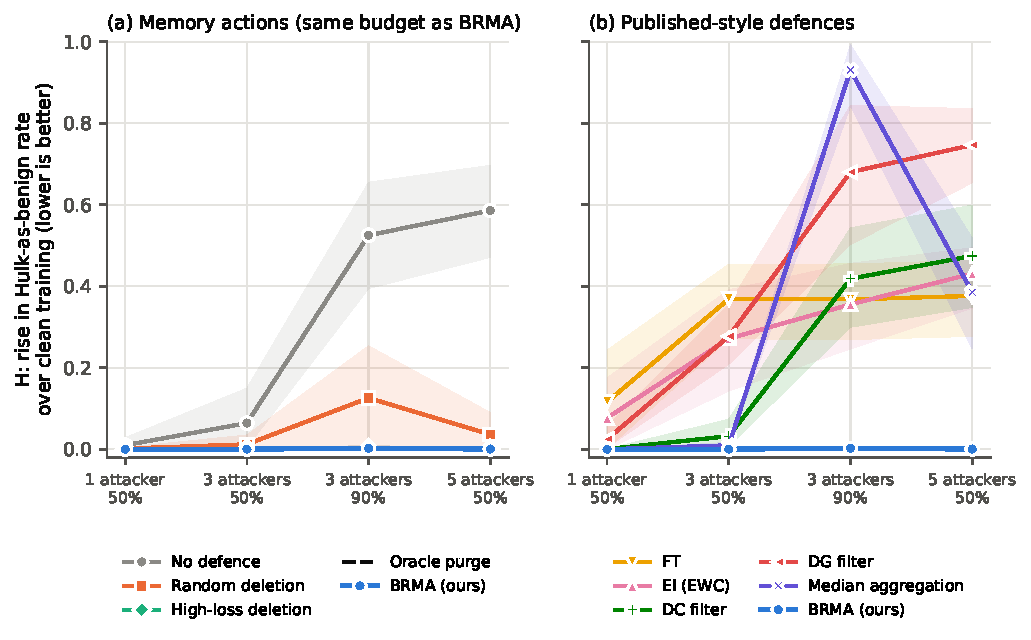
\includegraphics[width=\textwidth]{figures/fig2_attack_effect.pdf}
\caption{Attack effect $H$ against attack strength on CIC-IDS2017 (mean and 95\% bootstrap interval over 12 seeds). (a) Memory actions at the same removal budget as BRMA. (b) Published defences.}\label{fig:H}
\end{figure}

\begin{table}[htbp]
\caption{Pre-declared confirmatory tests on CIC-IDS2017 (one-sided paired Wilcoxon, 12 seeds, Holm correction over six). Wins: seeds on which BRMA is better (T6: seeds above the margin).}\label{tab:tests}
\footnotesize
\begin{tabularx}{\textwidth}{@{}lYccccc@{}}
\toprule
Test & Hypothesis & BRMA & Other & Wins & $p_{\mathrm{Holm}}$ & Result\\
\midrule
T1 & $H$: BRMA $<$ NONE at K3 & 0.0004 & 0.0643 & 12/12 & 0.0015 & confirmed\\
T2 & $H$: BRMA $<$ NONE at K3H & 0.0022 & 0.5251 & 12/12 & 0.0015 & confirmed\\
T3 & $H$: BRMA $<$ NONE at K5 & 0.0006 & 0.5857 & 12/12 & 0.0015 & confirmed\\
T4 & $H$: BRMA $<$ RAND at K3H & 0.0022 & 0.1260 & 12/12 & 0.0015 & confirmed\\
T5 & $H$: BRMA $<$ LOSS at K3H & 0.0022 & 0.0033 & 9/12 & 0.065 & not confirmed\\
T6 & clean macro-F1 non-inferior (margin 0.02) & 0.635 & 0.623 & 10/12 & 0.052 & not confirmed\\
\botrule
\end{tabularx}
\end{table}

\subsection{Utility of the protected learner}
Removing records must not cost legitimate learning. On clean data BRMA reaches 63.47\% macro-F1 against 62.29\% for NONE; the difference is $+1.18$ points with a bootstrap interval of $[-1.61, +4.26]$, inside the pre-declared margin, but the confirmatory test T6 narrowly misses significance after Holm correction ($p=0.052$, raw $p=0.026$), so we do not claim non-inferiority formally. The acquisition score is unchanged (39.4\% against 39.2\%), and the benign false-alarm rate rises from 6.5\% to 7.0\%. Under attack the audit improves utility: macro-F1 is 62.51\% against 59.00\% at K3H and 64.07\% against 58.62\% at K5 (paired $p=0.021$), and accuracy stays at 93.9--94.2\% in every arm while the undefended learner falls to 88.2\% at K5. Figure~\ref{fig:tradeoff} places every method in the robustness--utility plane under the strongest attack; BRMA, LOSS and ORACLE are the only methods that combine low $H$ with high macro-F1.

\begin{figure}[htbp]
\centering
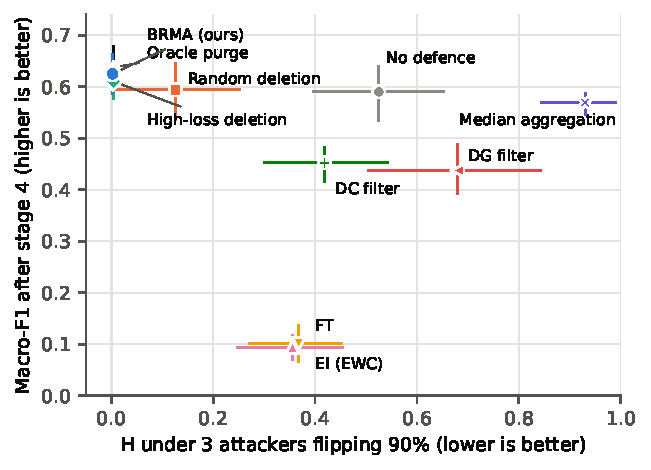
\includegraphics[width=0.72\textwidth]{figures/fig3_robustness_utility.pdf}
\caption{Robustness against utility under three attackers flipping 90\% of DoS Hulk (CIC-IDS2017, mean and 95\% interval).}\label{fig:tradeoff}
\end{figure}

\subsection{Audit quality and cost}
Table~\ref{tab:audit} and Figure~\ref{fig:audit} report the audit itself. After the attack stage BRMA flags 99.94--99.98\% of the poisoned records in memory on CIC-IDS2017, the second audit finds at most four remaining flipped records across all clients and seeds and removes them, so none remain at the end of the stream. The realised false-removal rate of genuine benign records is 4.5--4.7\% in every arm, below the level $\alpha=0.05$ as Proposition~\ref{prop:fdr} predicts, and about three genuine records per client are removed by the first audit. Because the false removals depend only on the benign side, the clean arm removes the same share as the attacked arms. Run time is unchanged within measurement noise (a mean difference of $-1$ s on 221 s per two-stage branch), and the statistics broadcast is one third of one model update once per stage.

\begin{table}[htbp]
\caption{Audit quality after the attack stage, summed over clients and seeds. Detection: poisoned records flagged; precision: flagged records that are poisoned; false removal: genuine benign records removed.}\label{tab:audit}
\footnotesize
\begin{tabularx}{\textwidth}{@{}lCCCCCC@{}}
\toprule
 & \multicolumn{3}{c}{CIC-IDS2017} & \multicolumn{3}{c}{TON\_IoT}\\
\cmidrule(lr){2-4}\cmidrule(l){5-7}
Arm & Detection & Precision & False removal & Detection & Precision & False removal\\
\midrule
C & -- & -- & 4.6\% & -- & -- & 5.0\%\\
K1 & 99.94\% & 90.8\% & 4.6\% & 55.9\% & 21.6\% & 5.0\%\\
K3 & 99.97\% & 97.3\% & 4.5\% & 56.5\% & 45.3\% & 5.0\%\\
K3H & 99.98\% & 98.4\% & 4.7\% & 58.2\% & 60.4\% & 5.0\%\\
K5 & 99.96\% & 98.3\% & 4.5\% & 58.4\% & 61.5\% & 5.0\%\\
\botrule
\end{tabularx}
\end{table}

\begin{figure}[htbp]
\centering
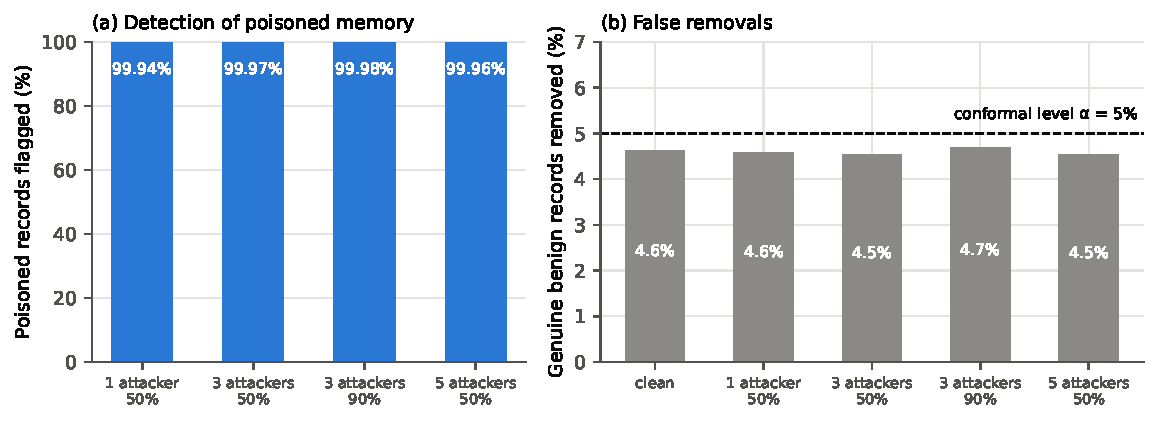
\includegraphics[width=\textwidth]{figures/fig4_audit_quality.pdf}
\caption{BRMA audit quality on CIC-IDS2017 after the attack stage. (a) Share of poisoned memory records flagged. (b) Share of genuine benign memory records removed, with the conformal level.}\label{fig:audit}
\end{figure}

\subsection{TON\_IoT and comparison with the state of the art}
Table~\ref{tab:ton} reports the TON\_IoT study. With the configuration selected on development seeds, the undefended learner reaches 88.84\% test macro-F1 on clean data (12 seeds, range 84.98--90.06\%) and BRMA 89.07\%, with 97.1\% accuracy. Under attack BRMA keeps 86.82\% (K3H) and 88.14\% (K5) macro-F1 against 81.84\% and 84.63\% for NONE (paired $p=0.001$ and $0.002$), and it reduces $H$ from 0.637 to 0.249 at K3H and from 0.496 to 0.194 at K5, winning on all 12 seeds. The reduction is smaller than on CIC-IDS2017, and DC (0.186) and LOSS (0.061) are lower at K3H. We analyse the reason in Section~\ref{sec:ablation}.

\begin{table}[htbp]
\caption{TON\_IoT, test split, mean over 12 seeds. Macro-F1 over all ten classes after the last stage.}\label{tab:ton}
\footnotesize
\begin{tabularx}{\textwidth}{@{}lCCCCCC@{}}
\toprule
 & \multicolumn{3}{c}{Macro-F1 (\%)} & Acc.\ (\%) & \multicolumn{2}{c}{$H$}\\
\cmidrule(lr){2-4}\cmidrule(lr){5-5}\cmidrule(l){6-7}
Method & C & K3H & K5 & C & K3H & K5\\
\midrule
NONE & 88.84 & 81.84 & 84.63 & 97.02 & 0.637 & 0.496\\
FT & 12.33 & 12.41 & 13.10 & 63.04 & 0.013 & 0.024\\
EI (EWC) & 33.13 & 26.55 & 28.59 & 76.03 & 0.311 & 0.327\\
DC & 87.92 & 85.44 & 87.10 & 96.74 & 0.186 & 0.118\\
DG & 51.43 & 47.92 & 45.30 & 85.36 & 0.547 & 0.603\\
MEDIAN & 89.77 & 80.26 & 86.31 & 97.44 & 0.888 & 0.499\\
RAND & 88.97 & 82.63 & 85.87 & 96.97 & 0.582 & 0.404\\
LOSS & 88.58 & 88.09 & 88.98 & 96.98 & 0.061 & 0.021\\
ORACLE & 88.84 & 88.34 & 89.50 & 97.02 & 0.045 & 0.013\\
BRMA (ours) & 89.07 & 86.82 & 88.14 & 97.10 & 0.249 & 0.194\\
\botrule
\end{tabularx}
\end{table}

Table~\ref{tab:sota} compares the best results reported by recent studies with ours. On TON\_IoT, the federated class-incremental system of Carillo et al.\ reports 74.49\% F1 over all classes (79.05\% on old and 68.10\% on new classes) \cite{carillo}, and EdgeFedCIL reports 80.77\% macro-F1 \cite{wu}. Our learner reaches 89.07\% (92.94\% old, 87.41\% new) with BRMA, 14.6 points above Carillo et al., and keeps 86.82\% under the strongest attack, which neither federated study evaluates. Only the centralised class-incremental system of Cerasuolo et al.\ reports a higher F1 on TON\_IoT (95.30\%) \cite{cerasuolo}, without federation or poisoning. The comparison has limits that we state explicitly. Carillo et al.\ and Cerasuolo et al.\ use packet-field inputs from the first packets of each flow, while we use flow features including the destination port; stage orders, client numbers and splits differ; and the values of other studies are as reported, not reproduced.

\begin{table}[htbp]
\caption{Comparison with the best results reported in recent studies. Values marked $^\ast$ are reported by the original authors and were not reproduced. Fed.: federated; CIL: class-incremental; Poison: evaluated under poisoning.}\label{tab:sota}
\footnotesize
\begin{tabularx}{\textwidth}{@{}p{3.1cm}p{2.2cm}cccY@{}}
\toprule
Study & Dataset & Fed. & CIL & Poison & Best reported result\\
\midrule
Carillo et al.\ 2026 \cite{carillo} & TON\_IoT & yes & yes & no & F1 all/old/new 74.49/79.05/68.10\%$^\ast$\\
Wu et al.\ 2026 \cite{wu} & ToN-IoT & yes & yes & no & macro-F1 80.77\%, accuracy 83.47\%$^\ast$\\
Cerasuolo et al.\ 2025 \cite{cerasuolo} & TON\_IoT & no & yes & no & F1 95.30\%$^\ast$ (packet fields)\\
Guo et al.\ 2025 \cite{guo} & CIC-IDS2017 & no & yes & no & accuracy 83.4\%, F1 82.1\%$^\ast$\\
Delgado et al.\ 2026 \cite{delgado} & CICIDS2017 and others & no & domain & no & macro-F1 0.92--0.98 (binary)$^\ast$\\
Wang et al.\ 2025 \cite{ctwa} & CICIoT2023 & no & yes & no & accuracy 96.43\%, F1 96.45\%$^\ast$\\
Lavaur et al.\ 2025 \cite{lavaur} & NF-UNSW-NB15, NF-CSE-CIC-IDS2018 & yes & no & yes & one of ten attackers: relative attack success well below 0.1, recovery after the attack$^\ast$\\
Sameera et al.\ 2025 \cite{wei} & federated NIDS benchmarks & yes & no & yes & target-class recall up to +70\%, F1 +1 to +14\%$^\ast$\\
Prasad et al.\ 2026 \cite{prasad} & CICIoT2023 (binary) & yes & no & yes & accuracy 97.96\%$^\ast$\\
This work, BRMA & CIC-IDS2017 & yes & yes & yes & accuracy 94.2\% and macro-F1 64.1\% with five attackers; attack effect 0.586 $\to$ 0.0006\\
This work, BRMA & TON\_IoT & yes & yes & yes & macro-F1 89.07\%, accuracy 97.10\% (clean); 86.82\% under three attackers flipping 90\%\\
This work, BRMA-C & TON\_IoT & yes & yes & yes & unseen seeds: macro-F1 88.98\% (clean), 88.62\% under three attackers flipping 90\%; attack effect 0.641 $\to$ 0.021\\
\botrule
\end{tabularx}
\end{table}

\subsection{Adaptive attackers}\label{sec:adaptive}
Table~\ref{tab:adaptive} reports the adaptive study. The selective attack is weaker than the standard attack without defence ($H=0.334$ against 0.525 at three attackers), because the most benign-looking Hulk records teach the model less about Hulk, but it does not evade the audit: BRMA still flags 99.98\% of the poisoned memory records and keeps $H$ at 0.0061 (S3H) and 0.0079 (S5), confirmed against NONE on all 12 seeds (T7, $p_{\mathrm{Holm}}=0.001$). The attacker's own score is estimated from its own traffic, and the records it selects as least suspicious still lie far above the server's benign calibration quantile. The loss-based memory action degrades under this attack: with BRMA's budget, LOSS removes 87.3\% of the poison at S5 and leaves $H=0.094$, against 0.008 for BRMA (exploratory $p_{\mathrm{Holm}}=0.009$).

The camouflage attack shows a trade-off for the attacker. Moving the flipped records half-way to benign traffic lowers BRMA's detection to 53.6\% (M3H) and 31.4\% (M5), but the moved records no longer resemble real DoS Hulk flows, and the attack effect without any defence falls to 0.0005, indistinguishable from clean training. T8 is therefore not confirmed: there is no effect left to remove. Within this threat model, an attacker can evade the feature-based audit only by giving up the poisoning effect.

The fixed-budget filter LOSS5 fails at every strong attack ($H=0.452$ at K3H and 0.313 at S3H), because 5\% of the memory is far less than the poisoned share; both tests against it are confirmed on all 12 seeds (T9, T10, $p_{\mathrm{Holm}}=0.001$). A loss ranking is useful only when it is told how many records to remove, which is what the conformal test provides.

\begin{table}[htbp]
\caption{Adaptive attackers on CIC-IDS2017, mean $H$ over 12 seeds (lower is better). S: selective attack against the audit; M: camouflage of flipped features ($\gamma=0.5$); K3H: standard attack for reference. The last row gives BRMA's detection of poisoned memory records after the attack stage.}\label{tab:adaptive}
\footnotesize
\begin{tabularx}{\textwidth}{@{}lCCCCC@{}}
\toprule
Method & K3H & S3H & S5 & M3H & M5\\
\midrule
NONE & 0.5251 & 0.3341 & 0.4499 & 0.0005 & 0.0006\\
RAND (matched budget) & 0.1260 & 0.1393 & 0.1851 & 0.0005 & 0.0003\\
LOSS (matched budget) & 0.0033 & 0.0289 & 0.0938 & 0.0007 & 0.0002\\
LOSS5 (fixed 5\%) & 0.4515 & 0.3135 & 0.4209 & 0.0013 & 0.0003\\
DC & 0.4184 & 0.3704 & 0.4682 & 0.0003 & 0.0001\\
MEDIAN & 0.9304 & 0.7583 & 0.4658 & 0.0011 & 0.0001\\
ORACLE (upper bound) & 0.0041 & 0.0072 & 0.0077 & 0.0009 & 0.0002\\
BRMA (ours) & 0.0022 & 0.0061 & 0.0079 & 0.0009 & 0.0002\\
\midrule
BRMA detection & 99.98\% & 99.98\% & 99.98\% & 53.6\% & 31.4\%\\
\botrule
\end{tabularx}
\end{table}

\subsection{Model-score and combined audits}\label{sec:variantres}
In phase 1 on TON\_IoT, all three variants met the eligibility rule, and the mean development $H$ under K3H and K5 was 0.012 for BRMA-M, 0.017 for BRMA-C, 0.104 for BRMA-G and 0.155 for BRMA; the rule therefore selected BRMA-M. Table~\ref{tab:variants} reports phase 2 on unseen seeds and the check on CIC-IDS2017.

On TON\_IoT, the model score resolves the overlap problem. BRMA-M detects 99.2--99.9\% of the poisoned records against 57--59\% for BRMA and lowers $H$ from 0.227 to 0.034 under K3H and from 0.217 to 0.0076 under K5; all four tests are confirmed (T11--T14, $p_{\mathrm{Holm}}=0.001$, 11--12 of 12 seeds). The false-removal rate stays at 4.9--5.2\%, and clean macro-F1 is 88.94\% against 88.74\% for NONE.

On CIC-IDS2017, BRMA-M fails under heavy poisoning. Its detection falls to 86.2\% under K3H, 76.5\% under S3H and 24.8\% under S5, and $H$ rises to 0.044, 0.085 and 0.343, against 0.002--0.008 for BRMA. T16 and T17 are confirmed, but non-inferiority to BRMA (T15, $p=0.55$) and on clean macro-F1 (T18, $p_{\mathrm{Holm}}=0.47$) are not. With tens of thousands of flipped DoS Hulk records, the global model learns to score Hulk as benign, so the model score of the flipped records is itself poisoned, as anticipated in Section~\ref{sec:variants}.

BRMA-C, which combines the contamination-free Gaussian test with the model score, is the only audit that is strong on both datasets. On TON\_IoT it detects 99.2--99.9\% of the poison and reaches $H=0.021$ under K3H and 0.0071 under K5, lower than BRMA on all 12 unseen seeds at K3, K3H and K5 (exploratory $p_{\mathrm{Holm}}=0.006$) and level with the oracle (0.021 and 0.011). On CIC-IDS2017 it detects 99.95--99.99\% and keeps $H$ at 0.0005--0.0079 in every arm, statistically indistinguishable from BRMA except under S3H, where BRMA is marginally lower (0.0061 against 0.0079). Its false-removal rate is 4.2--4.3\% on TON\_IoT and 4.1--4.8\% on CIC-IDS2017, within $\alpha$ as Proposition~\ref{prop:union} guarantees, and its clean macro-F1 differs from NONE by $+0.24$ points on TON\_IoT and $-0.33$ points on CIC-IDS2017, both within bootstrap intervals that include zero. The pre-specified rule selected BRMA-M on TON\_IoT alone; the recommendation of BRMA-C follows from the CIC-IDS2017 check and is therefore a post-hoc conclusion, although every BRMA-C value reported here comes from runs defined before the data were seen.

\begin{table}[htbp]
\caption{Model-score (BRMA-M) and combined (BRMA-C) audits. TON\_IoT: twelve unseen seeds (201--212), test split. CIC-IDS2017: main-study seeds, S = selective adaptive attack. $H$: attack effect (lower is better); Det.: poisoned memory records detected after the attack stage.}\label{tab:variants}
\footnotesize
\begin{tabularx}{\textwidth}{@{}lCCCCCCC@{}}
\toprule
 & \multicolumn{3}{c}{TON\_IoT} & \multicolumn{4}{c}{CIC-IDS2017}\\
\cmidrule(lr){2-4}\cmidrule(l){5-8}
Method & $H$ K3H & $H$ K5 & Det. & $H$ K3H & $H$ K5 & $H$ S5 & Det.\\
\midrule
NONE & 0.641 & 0.443 & -- & 0.525 & 0.586 & 0.450 & --\\
BRMA & 0.227 & 0.217 & 57--59\% & 0.0022 & 0.0006 & 0.0079 & $\ge$99.9\%\\
BRMA-G & 0.171 & 0.095 & 73\% & -- & -- & -- & --\\
BRMA-M & 0.034 & 0.0076 & $\ge$99.2\% & 0.044 & 0.074 & 0.343 & 25--99.9\%\\
BRMA-C & 0.021 & 0.0071 & $\ge$99.2\% & 0.0057 & 0.0005 & 0.0069 & $\ge$99.9\%\\
ORACLE & 0.021 & 0.011 & 100\% & 0.0041 & 0.0005 & 0.0077 & 100\%\\
\botrule
\end{tabularx}
\end{table}

\subsection{Ablation and failure analysis}\label{sec:ablation}
The memory controls act as an ablation of BRMA. ORACLE shows that the persistent damage on CIC-IDS2017 is carried by the memory, RAND shows that the removal budget alone does not explain the gain, and LOSS shows that, once the budget is fixed by BRMA, ranking by model loss is equally effective under the standard attack (T5 not confirmed, $H=0.0033$ against 0.0022). LOSS cannot set its own budget, however: under K3H about 75\% of the benign-labelled memory is poisoned, while in the clean arm none is, and only the conformal test distinguishes the two cases; with a fixed budget the loss filter fails (Section~\ref{sec:adaptive}). An additional observation, outside the tests specified in advance, is that the combination of the conformal budget with loss ranking is the best memory action on TON\_IoT, whereas BRMA's own ranking is more robust under the selective attack on CIC-IDS2017.

TON\_IoT exposes the limit predicted by Proposition~\ref{prop:power}. BRMA flags 56--58\% of the poisoned records there and none after the second audit, while LOSS removes 73--82\% with the same budget. Many DDoS flows in TON\_IoT have feature vectors close to normal flows, and 647 de-duplicated feature vectors occur with two different labels. The flipped records that BRMA misses are those whose Gaussian likelihood ratio does not exceed the benign calibration quantile, which is the overlap region in which Eq.~\eqref{eq:power} gives low power at a 5\% false-removal rate. Even ORACLE leaves $H=0.045$ at K3H, because part of the damage is learned from the poisoned stage data before any audit can act. The false-removal rate is 5.0\% after the first audit and 1.7\% after the second, consistent with Proposition~\ref{prop:fdr}. This limit of the Gaussian test is what BRMA-C removes (Section~\ref{sec:variantres}).

Figure~\ref{fig:class} shows the per-class F1 on CIC-IDS2017 under the strongest attack. BRMA restores DoS Hulk from 0.647 to 0.972 F1 and changes the other classes by small amounts that are not significant, the largest losses being DoS Slowhttptest ($-0.065$) and Slowloris ($-0.032$). Rare classes such as Bot (0.21) and PortScan (0.16) remain weak for every method; BRMA addresses poisoning, not the learning of rare families. On TON\_IoT, adding destination-port features raised development macro-F1 by 6--18 points depending on the learner setting (from 66.3\% to 84.5\% for the base setting), and a larger memory with more rounds raised it further to 87.6\%; these choices, made on development seeds, are the main source of the gain over the published result.

\begin{figure}[htbp]
\centering
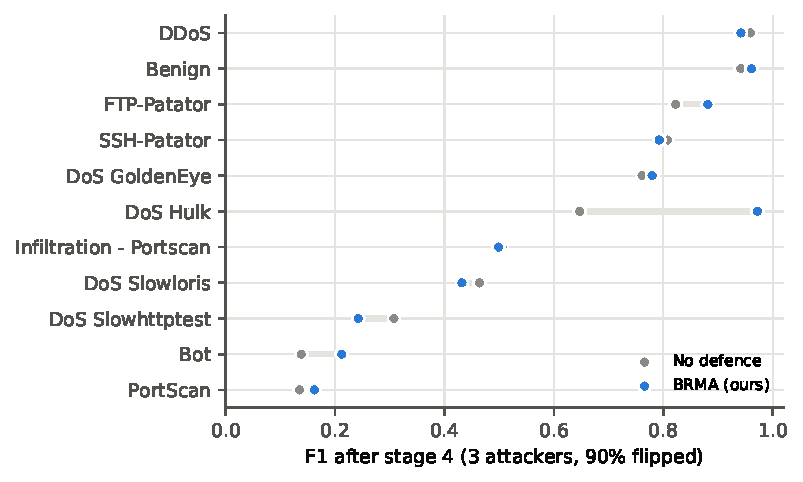
\includegraphics[width=0.72\textwidth]{figures/fig5_per_class.pdf}
\caption{Per-class F1 after the last stage on CIC-IDS2017 under three attackers flipping 90\% of DoS Hulk, without defence and with BRMA (mean over 12 seeds).}\label{fig:class}
\end{figure}

%=====================================================================
\section{Discussion}\label{sec:discussion}
The results support a simple view of the threat. In federated class-incremental learning the replay memory, not the aggregated model, is where label poisoning survives, and a defence that acts on the memory can remove it almost completely when the poisoned family is separable from benign traffic. BRMA needs no change to the learner or the aggregation, adds one statistics exchange per stage, and its false-removal rate is controlled by a single parameter with a finite-sample guarantee that held in every arm of both studies.

The scope of these findings is defined by the following assumptions. BRMA relies on clean first-stage benign records, the same trusted-bootstrap assumption made by FLTrust \cite{fltrust}; a deployment can satisfy it with a vetted reference capture. The adaptive attackers studied here select or camouflage records with their own copy of the audit; attackers that optimise feature perturbations jointly for evasion and poisoning effect, or that spread a smaller dose over several stages, form the next level of the threat model. The two studies of the model score also show a general design rule: an audit that relies only on the model being protected can be poisoned together with it, so a model-independent statistic should remain part of the decision, as in BRMA-C. The choice of BRMA-C over the pre-selected BRMA-M was made after the CIC-IDS2017 check and should be confirmed on further datasets. The simulation computes the server statistics from pooled data, and a deployment would obtain them through secure aggregation of the client sufficient statistics. CIC-IDS2017 results are reported on a held-out evaluation split that is not used for training, TON\_IoT results on a separate test split, and the comparison with published systems on TON\_IoT differs in input representation and protocol, as stated in Section~\ref{sec:results}. Five of the eighteen hypotheses specified in advance were not confirmed (T5, T6, T8, T15 and T18), and Section~\ref{sec:results} explains each case.

%=====================================================================
\section{Conclusion}\label{sec:conclusion}
We showed that label poisoning in federated class-incremental intrusion detection persists in client replay memories after the attackers withdraw, and proposed BRMA, a benign-reference likelihood-ratio audit with a conformal bound on false removals. On CIC-IDS2017 BRMA removed 99.9\% of poisoned memory records and reduced the attack effect of three to five coordinated clients from more than 0.5 to below 0.003, while keeping accuracy near 94\% and the false-removal rate below its 5\% level; adaptive attackers who select the most benign-looking records did not evade it, and camouflaged records evaded it only after losing their effect. On TON\_IoT the protected learner reached 89.07\% macro-F1, above the 74.49\% reported by Carillo et al. Where DDoS and normal flows overlap and the Gaussian test detected only 59\% of the poison, the combined audit BRMA-C raised detection above 99\% and reduced the attack effect to the level of an oracle on unseen seeds, while keeping the CIC-IDS2017 result; a model-only audit failed on CIC-IDS2017 because the model was poisoned with the data. Future work will evaluate attackers that optimise evasion and effect jointly, confirm BRMA-C on further datasets, and implement the statistics exchange with secure aggregation.

\backmatter

\section*{Declarations}
\begin{itemize}
\item Funding. No funding was received for this work.
\item Competing interests. The authors declare no competing interests.
\item Ethics approval and consent to participate. Not applicable. The study uses public benchmarks of network flows and involves no human participants.
\item Consent for publication. Not applicable.
\item Data availability. Both datasets are public: the corrected CIC-IDS2017 release (\url{https://intrusion-detection.distrinet-research.be/CNS2022/Datasets/CICIDS2017_improved.zip}) \cite{dataset,liu} and the TON\_IoT network data set (\url{https://research.unsw.edu.au/projects/toniot-datasets}) \cite{moustafa}. The preparation scripts rebuild every derived file from these sources.
\item Materials availability. Not applicable.
\item Code availability. The study code, the Kaggle notebooks, the per-run result records (2{,}715 runs) and the analysis scripts are available in the project repository (\url{https://github.com/ahmedbilalazhar/cl-ids-adversarial}).
\item Author contribution. Both authors designed the study. Saneedullah designed BRMA and the adaptive attacks, ran the CIC-IDS2017 and TON\_IoT studies, produced the analysis and figures, and drafted the manuscript. Ahmed Bilal built the reference data pipeline and the audited federated continual-learning engine on which all studies run, and reviewed the manuscript. Both authors read and approved the final manuscript.
\item AI-tool usage. AI assistants (Claude by Anthropic) were used to support code development, to generate analysis scripts and to edit the language of this text. The authors specified the research design, ran the experiments, checked the reported numbers against the stored result files and the literature figures against the cited sources, and take full responsibility for the content.
\end{itemize}

\bibliography{sn-bibliography}

\end{document}
